\section{PHƯƠNG TRÌNH ĐƯỜNG THẲNG}

\subsubsection{Phương trình tổng quát của đường thẳng}

\immini{\iconMT\indam{Véc tơ pháp tuyến:} Véc-tơ $\overrightarrow{n} \ne \vec{0}$ được gọi là véc-tơ pháp tuyến (vtpt) của đường thẳng $\Delta $ nếu giá của $\overrightarrow{n}$ vuông góc với $\Delta $ (hình vẽ).\begin{tcolorbox}[colframe=orange,colback=orange!4!,boxrule=0.2mm]
			\begin{itemize}
				\item  Một đường thẳng có vô số véc-tơ pháp tuyến và chúng cùng phương nhau.
				\item  Nếu $\overrightarrow{n}$ và $\overrightarrow{n'}$ cùng là véc-tơ pháp tuyến của $\Delta$ thì $\overrightarrow{n'}$=$k \cdot \overrightarrow{n}$.
				\item  Đường thẳng $\Delta$ hoàn toàn xác định khi biết một điểm và một véc tơ pháp tuyến của nó.
			\end{itemize}
		\end{tcolorbox}
	}{%\vspace{1.8cm}
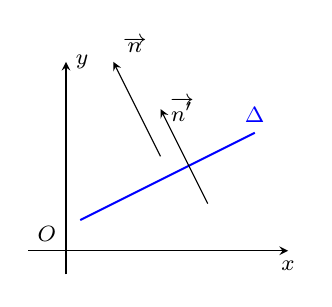
\begin{tikzpicture}[smooth,samples=300,scale=0.6,>=stealth,font=\footnotesize]
			\draw[->] (-0.8,0)--(4.7,0) node[below]{$x$};
			\draw[->] (0,-0.5)--(0,4) node[right]{$y$};
			\draw (0,0) node[above left]{$O$};
			\draw[line width=0.7pt, blue,domain=0.3:4] plot(\x,{0.5*((\x)+1)})node[above]{$\Delta$};
			\draw[->] (2,2)--(1,4) node[above right]{$\overrightarrow{n}$};
			\draw[->] (3,1)--(2,3) node[right]{$\overrightarrow{n'}$};
\end{tikzpicture}
}

\immini{
\iconMT \indam{Phương trình tổng quát của đường thẳng:} 
Trong mặt phẳng toạ độ, mọi đường thẳng đều có phương trình tổng quát dạng $ax+by+c=0$, với $a$, $b$ không đồng thời bằng $0$. Khi đó một véc tơ pháp tuyến của đường thẳng là $\vec{n}=(a;b)$.
}{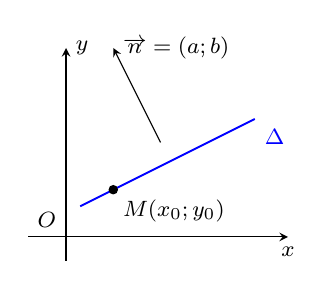
\begin{tikzpicture}[smooth,samples=300,scale=0.6,>=stealth,font=\footnotesize]
	\draw[->] (-0.8,0)--(4.7,0) node[below]{$x$};
	\draw[->] (0,-0.5)--(0,4) node[right]{$y$};
	\draw (0,0) node[above left]{$O$};
	\draw[line width=0.7pt, blue,domain=0.3:4] plot(\x,{0.5*((\x)+1)})node[below right]{$\Delta$};
	\draw[->] (2,2)--(1,4) node[right]{$\overrightarrow{n}=(a;b)$};
	\draw[fill=black] (1,1) circle (2.5pt) node[below right]{$M(x_0;y_0)$};
\end{tikzpicture}
}

\vspace{-0.5cm}

\iconMT \indam{Lưu ý:} \\
\begin{itemize}
	\item [\ding{172}] Đường thẳng $\Delta \colon \heva{& \text{ qua } M(x_0;y_0) & (1)\\& \text{vtpt } \overrightarrow{n}=\left(a;b\right)& (2)}$ sẽ có phương trình tổng quát là 
	\boxmini{$a(x-x_0)+b(y-y_0)=0$ \quad $(\star)$}
	ta thu gọn $(\star)$ về dạng $ax+by+c=0$.
	\item [\ding{173}] Cho $\Delta \colon ax+by+c=0$. 
	\begin{itemize}
		\item [$\bullet$] Nếu $b=0$ thì $\Delta$ có thể đưa về dạng $x=-\dfrac{c}{a}$ (vuông góc với $Ox$).
		\item [$\bullet$] Nếu $b \ne 0$, chia hai vế cho $b$ thì $\Delta$ có thể đưa về dạng $y=-\dfrac{a}{b}x-\dfrac{c}{b}$.
	\end{itemize}	
\end{itemize}



\subsubsection{ Phương trình tham số của đường thẳng}
\immini{
\iconMT \indam{Véc tơ chỉ phương: }Véc-tơ $\overrightarrow{u} \ne \vec{0}$ được gọi là véc-tơ chỉ phương (vtcp) của đường thẳng $\Delta $ nếu giá của $\overrightarrow{u}$ song song hoặc trùng với $\Delta $.\\
	\begin{tcolorbox}[colframe=orange,colback=orange!4!,boxrule=0.2mm]
		\begin{itemize}
			\item  Một đường thẳng có vô số véc-tơ chỉ phương và chúng cùng phương với nhau.	
			\item  Đường thẳng $\Delta$ hoàn toàn xác định khi biết một điểm và một véc tơ chỉ phương của nó.
		\end{itemize}
	\end{tcolorbox}
}{%\vspace{-0.8cm}
	\begin{tikzpicture}[smooth,samples=300,scale=0.7,>=stealth,font=\footnotesize]
		\draw[->] (-0.8,0)--(5,0) node[below]{$x$};
		\draw[->] (0,-0.5)--(0,4) node[right]{$y$};
		\draw (0,0) node[above left]{$O$};
		\draw[magenta,line width=0.7pt,domain=0.3:4] plot(\x,{0.5*((\x)+1)})node[above]{$\Delta$};
		\draw[->,blue] (1,2)--(3,3) node[above]{$\overrightarrow{u}$};
		\draw[->,violet] (1,0.5)--(4,2) node[below right]{$\overrightarrow{u'}$};
		\node[below] at (2,-1.3) {Nếu $\overrightarrow{u}$ và $\overrightarrow{u'}$ là véc-tơ chỉ phương}; 
		\node[below] at (2,-2.3) {của $\Delta$ thì $\overrightarrow{u}=k \cdot \overrightarrow{u}$.}; 
	\end{tikzpicture}
}
\vspace{0.8cm}

\iconMT \indamm{Mối liên hệ giữa véc tơ chỉ phương và véc tơ pháp tuyến:} \\
Cho $\vec{n}=(a;b)$ là một véc tơ pháp tuyến của $\Delta$. Khi đó $\Delta$ có một véc tơ chỉ phương là $\vec{u}=(-b;a)$ hoặc $\vec{u}=(b;-a)$ (đổi chỗ và đổi 1 dấu).

\vspace{0.8cm}

\iconMT \indam{Phương trình tham số của đường thẳng:} \\
Đường thẳng $\Delta \colon \heva{& \text{ qua } M(x_0;y_0) & (1)\\& \text{vtcp } \overrightarrow{u}=\left(u_1;u_2\right)& (2)}$ sẽ có phương trình tham số là \boxmini{$\heva{&x=x_0+u_1t\\&y=y_0+u_2t}\quad (t \in \mathbb{R})$}

\subsubsection{Mối liên hệ giữa đồ thị hàm bậc nhất và đường thẳng}
\begin{listEX}[1]
	\item [\ding{172}] Đồ thị hàm số bậc nhất $y=kx+y_0$ là một đường thẳng có hệ số góc $k$ có thể được viết thành $kx-y+y_0$. Suy ra một véc tơ pháp tuyến là $\vec{n}=(k;-1)$.
	\begin{boxdn}
		\indam{Ghi nhớ:} Một đường thẳng có hệ số góc $k$ thì nó sẽ có một véc tơ pháp tuyến là $\vec{n}=(k;-1)$.
	\end{boxdn}
	\vspace{0.8cm}
	\item [\ding{173}] Ngược lại, mỗi đường thẳng có phương trình $ax+by+c=0$, với $a,\,b \ne 0$ có thể được viết thành dạng hàm số bậc nhất $y=-\dfrac{a}{b}x-\dfrac{c}{b}$.
\end{listEX}

\newpage

\subsubsection{ Vị trí tương đối của hai đường thẳng}
Cho hai đường thẳng $\heva{&{\Delta}_1\colon a_1x+b_1y+c_1=0\\&{\Delta}_2 \colon a_2x+b_2y+c_2=0}$. Để kiểm tra vị trí tương đối giữa chúng, ta có thể làm theo một trong hai cách sau:
\begin{itemize}
	\item [\iconMT] \indam{Cách 1: Dựa vào số nghiệm của hệ phương trình.}\\
	Xét hệ $\heva{
		& a_1x+b_1y+c_1=0 \\ 
		& a_2x+b_2y+c_2=0 \\}.$
	\begin{boxkn}
		\begin{itemize}
			\item Nếu hệ có một nghiệm $\left(x_0;y_0\right)$ thì ${\Delta}_1$ cắt ${\Delta}_2$ tại điểm $M_0\left(x_0;y_0\right).$
			\item Nếu hệ có vô số nghiệm thì ${\Delta}_1$ trùng với ${\Delta}_2$.
			\item Nếu hệ vô nghiệm thì ${\Delta}_1$ và ${\Delta}_2$ không có điểm chung, hay ${\Delta}_1$ song song với ${\Delta}_2$.
		\end{itemize}
	\end{boxkn}
	\item [\iconMT] \indam{Cách 2: Xét tỉ số (với $a_2$, $b_2$, $c_2$ khác 0)}
	\begin{boxkn}
		\begin{itemize}
			\item Nếu $\dfrac{a_1}{a_2}=\dfrac{b_1}{b_2}=\dfrac{c_1}{c_2}$ thì ${\Delta}_1$ trùng với ${\Delta}_2$.
			\item Nếu $\dfrac{a_1}{a_2}=\dfrac{b_1}{b_2}\ne \dfrac{c_1}{c_2}$ thì ${\Delta}_1$ song song ${\Delta}_2$.
			\item  Nếu $\dfrac{a_1}{a_2}\ne \dfrac{b_1}{b_2}$ thì ${\Delta}_1$ cắt ${\Delta}_2$.
		\end{itemize}
	\end{boxkn}
\end{itemize}

\subsubsection{ Góc giữa hai đường thẳng}
\begin{itemize}
	\item [\iconMT] \indam{Công thức tính:} Cho hai đường thẳng 
	${\Delta}_1\colon a_1x+b_1y+c_1=0$ và 
	${\Delta}_2\colon a_2x+b_2y+c_2=0$.  Gọi $\varphi $ $(0^\circ \le \varphi \le 90^\circ)$ là góc tạo bởi giữa hai đường thẳng ${\Delta}_1$ và ${\Delta}_2$.
	Khi đó
	\boxmini{$\cos \varphi =\left| \cos \left(\overrightarrow{n_1},\overrightarrow{n_2}\right)\right|=\dfrac{\left| \overrightarrow{n_1}\cdot\overrightarrow{n_2}\right|}{\left| \overrightarrow{n_1}\right|\cdot \left| \overrightarrow{n_2}\right|}=\dfrac{\left| a_1\cdot a_2+b_1\cdot b_2\right|}{\sqrt{a_1^2+b_1^2}\cdot\sqrt{a_2^2+b_2^2}}.$}
	với $\overrightarrow{n_1}=\left(a_1;b_1\right)$, $\overrightarrow{n_2}=\left(a_2;b_2\right)$ lần lượt là vtpt của $\Delta_1$ và $\Delta_2$.
	\immini{
		\item[\iconMT] \indam{Chú ý: }
		\begin{boxkn}
			\begin{itemize}
				\item [$\bullet$] $0^\circ \le \varphi \le 90^\circ$.
				\item [$\bullet$] Nếu $\Delta_1$ song song hoặc trùng $\Delta_2$ thì $\varphi=0^\circ$.
				\item [$\bullet$] Nếu $\Delta_1$ vuông góc $\Delta_2$ thì $\varphi=90^\circ$ hay \fbox{$a_1a_2+b_1b_2=0$}.
			\end{itemize}
	\end{boxkn}}{
		\begin{tikzpicture}[scale=0.7, line join=round, line cap=round]
			\tkzDefPoints{0/0/A,4/0/B,0.5/-0.5/C,4/3/D,1/0/M}
			\tkzDrawSegments(A,B D,C)
			%\tkzMarkAngles[size=0.7cm,arc=ll](B,M,D)
			\tkzLabelAngles[pos=1,rotate=30](B,M,D){$\varphi$}
			\tkzDrawPoints[size=3,fill=black](M)
			\draw (4,0)node[below]{$\Delta_1$} (4,3)node[below right]{$\Delta_2$};
			\begin{scope}
				\clip (D)--(M)--(B);
				\draw[double] (M) circle(0.6cm);
			\end{scope}
	\end{tikzpicture}}
\end{itemize}

\newpage

\subsubsection{ Khoảng cách từ một điểm đến một đường thẳng}
\immini{ \iconMT \indam{Công thức tính:} Khoảng cách từ $M_0\left(x_0;y_0\right)$ đến đường thẳng $\Delta\colon ax+by+c=0$ được tính theo công thức
		\boxmini{$d\left(M_0,\Delta \right)=M_0H=\dfrac{\left| ax_0+by_0+c\right|}{\sqrt {a^2+b^2}}$}
}{\hspace{1.5cm}
		\begin{tikzpicture}[scale=1, line join=round, line cap=round]
			\draw[-] (0,0)--(4,0) node [below]{$\Delta$};
			\draw[-] (2,0)node [below]{$H$}--(2,1.5) node [right]{$M_0$};
			\draw[fill=black] (2,0) circle(1.5pt) (2,1.5) circle(1.5pt);
	\end{tikzpicture}
}
\iconMT \indam{Các trường hợp đặc biệt:} $d\left(M_0,Ox \right)=M_0H=\big|y_0\big|$, \quad $d\left(M_0,Oy \right)=M_0K=\big|x_0\big|$. \\
\iconMT \indam{Phương trình các đường phân giác góc tạo bởi hai đường thẳng cắt nhau:}\\
Cho hai đường thẳng $\Delta_1\colon a_1x+b_1y+c_1=0$ và ${\Delta}_2\colon a_2x+b_2y+c_2=0$ cắt nhau thì phương trình hai đường phân giác của góc tạo bởi hai đường thẳng trên là
	$$\dfrac{a_1x+b_1y+c_1}{\sqrt{a_1^2+b_1^2}}=\pm \dfrac{a_2x+b_2y+c_2}{\sqrt{a_2^2+b_2^2}}$$

\begin{dang}{Phương trình tổng quát của đường thẳng}
	\indam{Xét phương trình tổng quát:} Cho $\Delta \colon ax+by+c=0$ thì
	\begin{itemize}
		\item [$\bullet$] Một vtpt là $\overrightarrow{n}=(a,b)$ (hệ số của $x$ và $y$.)
		\item [$\bullet$] Tìm điểm thuộc $\Delta$: Cho trước $x$, thay vào phương trình tìm $y$ hoặc ngược lại.
	\end{itemize}
\end{dang}

\begin{dang}{Phương trình tham số của đường thẳng}
	\indam{Xét phương trình tham số:} Cho $\Delta \colon \heva{&x=x_0+u_1t\\&y=y_0+u_2t}$ thì
	\begin{itemize}
		\item [$\bullet$] Một vtcp là $\overrightarrow{u}=(u_1;u_2)$ (hệ số của $t$.)
		\item [$\bullet$] Tìm điểm thuộc $\Delta$: Cho trước $t$, thay vào phương trình tìm $x$ và $y$.
	\end{itemize}
	
\end{dang}

\begin{dang}{Chuyển phương trình tham số về phương trình tổng quát và ngược lại}
	\indam{Mối liên hệ giữa véc tơ chỉ phương và véc tơ pháp tuyến:} Cho $\vec{n}=(a;b)$ là một véc tơ pháp tuyến của $\Delta$. Khi đó $\Delta$ có một véc tơ chỉ phương là $\vec{u}=(-b;a)$ hoặc $\vec{u}=(b;-a)$ (đổi chỗ và đổi 1 dấu).
\end{dang}

\begin{dang}{Lập phương trình đường thẳng đi qua hai điểm phân biệt cho trước}
	\begin{itemize}
		\item [\iconMT] Trong mặt phẳng $Oxy$, cho hai điểm $A(x_A;y_A)$ và $B(x_B;y_B)$. Khi đó, đường thẳng $AB$ sẽ có một véc tơ chỉ phương là $\vec{AB}=(x_B-x_A;y_B-y_A)$.
		\item [\iconMT] \indam{Lưu ý:}
		\begin{itemize}
			\item [$\bullet$] Nếu $x_B-x_A \ne 0$ và $y_B-y_A \ne 0$ thì phương trình $AB$ là
			$\dfrac{x-x_A}{x_B-x_A}=\dfrac{y-y_A}{y_B-y_A}$.
			\item [$\bullet$] Nếu $A(a;0)$ và $B(0;b)$, với $a,b \ne 0$ thì phương trình $AB$ là $\dfrac{x}{a}+\dfrac{y}{b}=1$.
		\end{itemize}
	\end{itemize}
\end{dang}

\begin{dang}{Các bài toán liên quan đến hình chiếu và đối xứng}
	\begin{itemize}
		\item [\iconMT] \indam{Bài toán 1:} Tìm hình chiếu của điểm $M(x_0;y_0)$ lên $\Delta \colon ax+by+c=0$.
		\immini{
			\begin{itemize}
				\item [$\bullet$] Gọi $H$ là hình chiếu vuông góc của $M$ lên $\Delta$.
				\item [$\bullet$]  Do $MH \perp \Delta$ nên phương trình $MH$ có dạng $bx -ay+m=0 \quad (1)$. Thay tọa độ $M$ vào (1), tìm $m$.
				\item [$\bullet$] Nhận xét $H=MH \cap \Delta$ nên tọa độ $H$ là nghiệm của hệ $\heva{&ax+by+c=0\\&bx-ay+m=0} \quad(2)$
				\item [$\bullet$] Giải (2), tìm nghiệm $(x_1;y_1)$. Kết luận $H(x_1;y_1)$.
		\end{itemize}}{\hspace{2cm}
			\begin{tikzpicture}[scale=1, line join=round, line cap=round]
				\draw (0,0)--(4,0) node [below]{$\Delta$};
				\draw[dashed] (2,-1.5)node [below right]{$M'$}--(2,0);
				\draw (2,0)node [below right]{$H$}--(2,1.5) node [right]{$M(x_0;y_0)$};
				\draw[fill=black] (2,0) circle(1.5pt) (2,1.5) circle(1.5pt) (2,-1.5) circle(1.5pt);
		\end{tikzpicture}}
		\item [\iconMT] \indam{Bài toán 2:} Tìm tọa độ điểm $M'$ đối xứng với điểm $M(x_0;y_0)$ qua $\Delta \colon ax+by+c=0$.
		\begin{itemize}
			\item [$\bullet$] Gọi $M'(x';y')$ là điểm đối xứng với $M$ qua $\Delta$.
			\item [$\bullet$] Khi đó, $H$ là trung điểm của đoạn $MM'$.
			Suy ra, tọa độ $M'$ được tính theo công thức sau $$\heva{&x'=2x_1-x_0\\&y'=2y_1-y_0}$$
		\end{itemize}
	\end{itemize}
\end{dang}

\begin{dang}{Tìm điểm $M$ thỏa mãn điều kiện cho trước}
	Để xác định tọa độ điểm $M$, ta thường tiếp cận theo hai cách sau:
	\begin{itemize}
		\item [\iconMT] \indam{Cách 1:} Tham số tọa độ điểm $M$ theo ẩn. Sau đó, kết hợp với giả thiết để xây dựng phương trình giải. Các kiểu tham số điểm thường gặp:
		\begin{tcolorbox}[colframe=orange,colback=red!2!white,boxrule=0.2mm]
			\begin{itemize}
				\item Nếu $M \in Ox$ thì $M(m;0)$.
				\item Nếu $M \in Oy$ thì $M(0;m)$.
				\item Nếu $M \in \Delta \colon \heva{&x=x_0+u_1t\\&y=y_0+u_2t}$ thì $M\bigg(x_0+u_1t;y_0+u_2t\bigg)$.
				\item Nếu $M \in \Delta \colon ax+by+c=0$ thì $M\bigg(x_0;\dfrac{-c-ax_0}{b}\bigg)$, với $b \ne 0$.
			\end{itemize}
		\end{tcolorbox}
		\begin{luuy}
			Chú ý các công thức tính độ dài, tính góc, khoảng cách; điều kiện vuông góc,...
		\end{luuy}
		\item [\iconMT] \indam{Cách 2:} Điểm $M$ có thể là giao của hai "đối tượng" hình nào đó trong đề bài (giao của hai đường thẳng, giao của đường thẳng với đường tròn,...). Khi đó, ta viết phương trình của hai "đối tượng" hình đó, rồi giải hệ tìm kết quả.
	\end{itemize}
\end{dang}